\documentclass{article}

\usepackage[margin=1in]{geometry}
\usepackage{graphicx}
\usepackage{listings}
\usepackage{siunitx}
\usepackage{float}





\begin{document}

\begin{verbatim}
a =
   364
b =
  -228
c =
   2.0000 + 5.0000i
d =
  -3.0000 - 4.0000i
calc_1 =
  183.4692
S =
 -26.0000 - 7.0000i
Real_S =
   -26
Imag_S =
    -7
Mag_S =
   26.9258
Ang_S_rad =
   -2.8786
Ang_S_deg =
 -164.9315
F =
   0.2145 - 0.1172i

-------------------------- Part 3 ---------------------------

restistors = [133.4000,  162.3000,  158.7000,  148.1000,  154.2000,  141.6000,  147.5000]
R_avg =
  149.4000
R_median =
  148.1000
R_min =
  133.4000
R_max =
  162.3000
R_Sd =
    9.9840


\end{verbatim}
$
I_0 = 46 \si{mA}\\
\tau = 15.9174 \si{s}
$

\medskip
 \begin{figure}[H]
  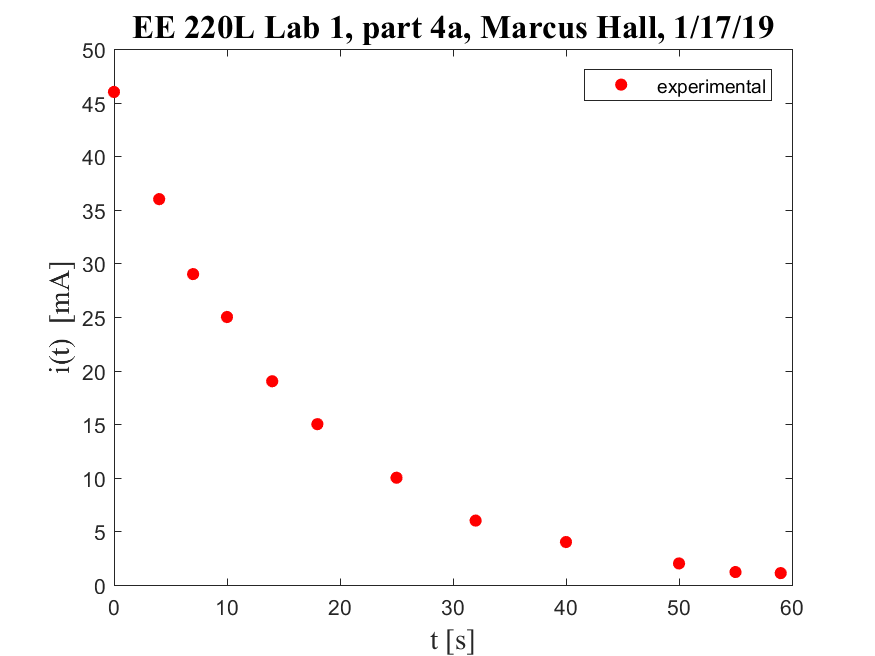
\includegraphics[width=4in]{lab_1_4a.png}
  \caption{Part 4a}
  \label{fig:4a}
\end{figure}

\begin{figure}[H]
  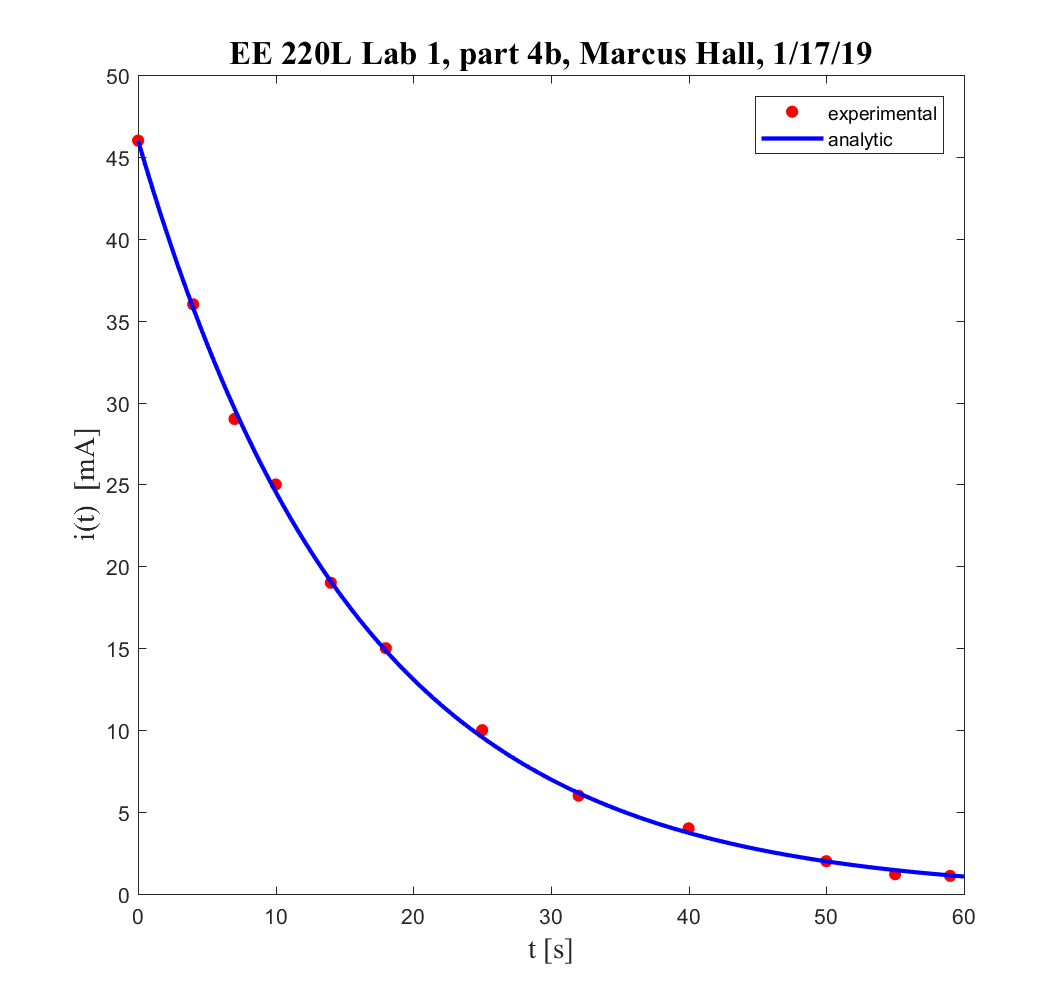
\includegraphics[width=4in]{lab_1_4b.png}
  \caption{Part 4a}
  \label{fig:4a}
\end{figure}

\pagebreak

\lstinputlisting[caption={MATLAB code for Lab 1 Circuits 1},
 label={code:lab_1}, frame=tb]{Lab_1_Part_4.m}

\begin{lstlisting}

\end{lstlisting}

\end{document}